% Chapter 5

\chapter{Software Module Implementation}
\label{Chapter 5}
%\head{}

\section{Overview}
This chapter explains how each of the modules discussed in the previous chapter are implemented in software. First, the WiSARD Browser is discussed. The command generator module will be discussed next, followed by the validation module. The validation module is discussed last, as it has the broadest impact on the other modules and the system as a whole. 

\section{WiSARD Browser}
The WiSARD Browser module is a collection of software components which address four major objectives.

\begin{itemize}
	\item Allow a user to specify WiSARD search parameters through a user interface
	\item Search the WiSARDNet PostgreSQLdatabase for WSN state information
	\item Produce a set of WiSARD data objects matching the search criteria specified by the user
	\item The module should integrate with the existing WiSARDNet software
\end{itemize}

% flow of execution - wisard browser module
Figure \ref{fig:wisard_browser_flow} shows the flow of execution for this module. Each procedure shown is described in this chapter.

\begin{figure}[H]
	\centering
	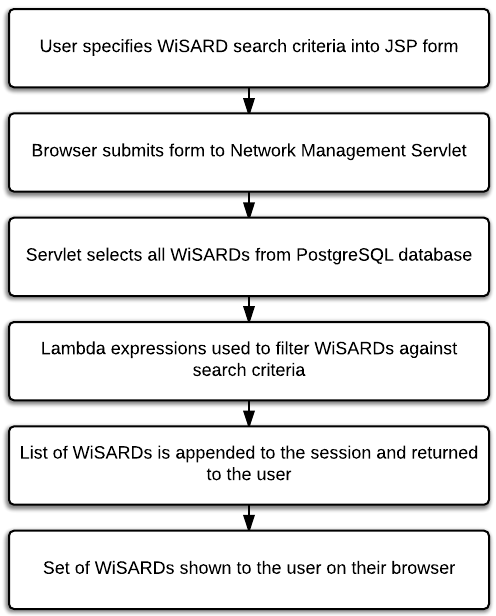
\includegraphics[width=0.6\textwidth]{figures/flow_diagram_wisard_browser.png}
	\caption{A flow diagram showing each action the WiSARD Browser Module  makes}
	\label{fig:wisard_browser_flow}
\end{figure}

\subsection{Obtaining the User's Search Criteria}
A user of this system needs to have an interface with which to send and receive information. To create this interface, JSP (JavaServer Pages) and Java servlets are used. A JSP page can present information to a user through a web browser as well as gather user input necessary for back-end operations. The JSP page can send information back and forth with a servlet which is a java class that implements methods to respond to Get and Post requests from a web browser. Figure \ref{fig:jsp_interaction} shows how a servlet is used to deliver information from the users to the appropriate software module, and vice versa. 

\begin{figure}[H]
	\centering
	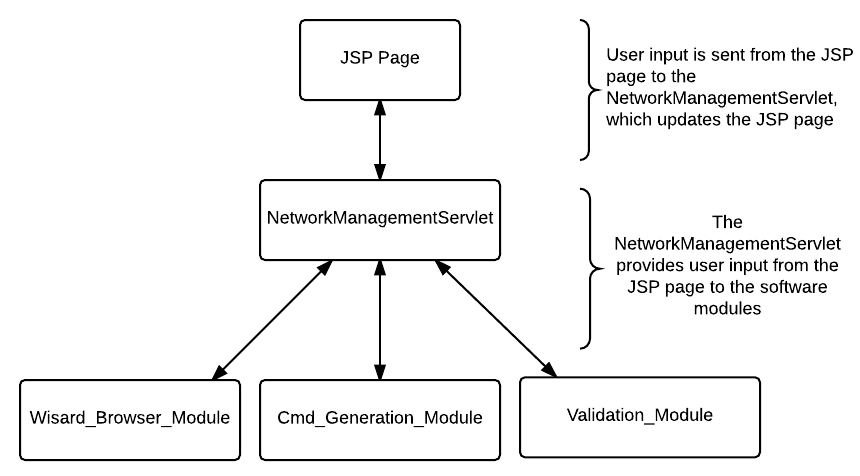
\includegraphics[width=\textwidth]{figures/jsp_interaction.png}
	\caption{A depiction of the way in which the servlet relays information between the user interface and the core software modules }
	\label{fig:jsp_interaction}
\end{figure} 

A JSP web page provides a simple interface for the user to populate an HTML form with attributes that can be used to select a set of WiSARDs:

\begin{itemize}
	\item WiSARD Network ID
	\item Device Serial ID
	\item Garden Site
	\item Associated Experiment
	\item SP type
	\item Transducer type
	\item WiSARD role
	\item Deployment Type
\end{itemize} 

These attributes are are static or dynamic pieces of information that together represent the current state of the WSN nodes. Traditionally, this information can be obtained from a database query that can be written into a function or a method. With the functional needs of the WiSARDs changing, and the types of experimentation that WiSARDNet will perform still in development, it is important for the this software to be flexible and support changes to the system. For example, if new WiSARD features are added, resulting in new fields in a PostgreSQL table, the new features should not prompt extensive modification of the existing code.\\

PostgreSQL supports a wide variety of query features that enable sophisticated data processing and filtration of queried data sets. If achieving the fasted possible query speed was of great importance for this module, then all of the searching and filtration of WiSARDs from the user's search criteria should be handled by complex PostgreSQL queries. While query time is important, the benefits that can be gained at the sacrifice of a small amount of processing speed make other solutions desirable. Chapter 2 briefly explained some of the ways in which modern software development techniques such as behavioral parameterization can add value to software. For the WiSARD browser module, a functional data processing approach would not only allow for this module to meet the needs of the system, but would allow for development flexibility at the expense of some very minor performance overhead. This does not impact the performance of the system in a significant way is because the amount of WiSARD state information compared to the amount of data stored in the database is trivial.\\

WiSARD data objects translate well from design concept to a practical software entity. A Java class with member variables that correspond to the different attributes that define a WiSARD's state, and methods to translate higher-level queries into database queries and results provides a foundation for objects to be created and passed from module to module. To achieve the desired flexibility, the module performs a single fetch to the database and retrieves all of the state information for all of the WiSARDs. It then formats the information from the query into WiSARD objects before adding them to a list data structure. All of this functionality is built into the WiSARD class.\\

Once the servlet has obtained a list of all WiSARD objects, it can then filter that list against the attributes which the user specified in his/her form submission. Utilizing functional data processing techniques supported by lambda expressions in Java 8, obtaining a list that matches a user's search criteria is simple and flexible. Below is an example of the way in which lambda expressions are used in this software to produce powerful results with a very small amount of code.\\ 

\begin{lstlisting}
return wisards.where((Wisard w) -> ''Arboretum''.equals(w.getSite()));
\end{lstlisting}

This statement returns an ArrayList named \textit{wisards} that contains WiSARD objects. The \textit{where()} method iterates over every entry in the ArrayList and only returns those who are not filtered out against the logic in the lambda expression. The lambda expression in this example compares the WiSARD site against a string containing the site name \textit{Arboretum}. Any WiSARD in the ArrayList that does not have \textit{Arboretum} as its site name will not be added to the ArrayList that is returned.\\

With one line of code, a data structure of WiSARD objects can  be filtered based on its member variables that would otherwise have required a specific database query. Additionally, values can be added to the same expression to create more complex data filtration without requiring that the underlying functionality be altered. This functionality provides a quick and versatile way to support changing project requirements for managing networks of WiSARDs without being restricted by specific database queries.\\

When a list of WiSARDs has been filtered to match a user's search, the servlet appends it to the browser session where it is accessible to the JSP page. The JSP page displays the WiSARDs and their state information for the user. From this point a user can decide to continue with reconfiguring the WiSARDs that this search has returned, or return to the form and specify a different set of WiSARDs. Should the user choose to continue on with the set of WiSARDs they have selected, the data structure is accessible within the browser session, ready to send to the command module.\\

\section{Command Generation}
The command generation module is similar to the WiSARD browser module, in that it relies on user input being sent from the JSP page to the servlet. The user will utilize the same JSP page's user interface as the WiSARD browser to select the change he/she would like to apply to the selected WiSARDs. Figure \ref{fig:flow_cmd_generator} shows the flow of execution for this module. Each procedure shown in the diagram is described in this section.\\

% flow of execution, cmd module
\begin{figure}[H]
	\centering
	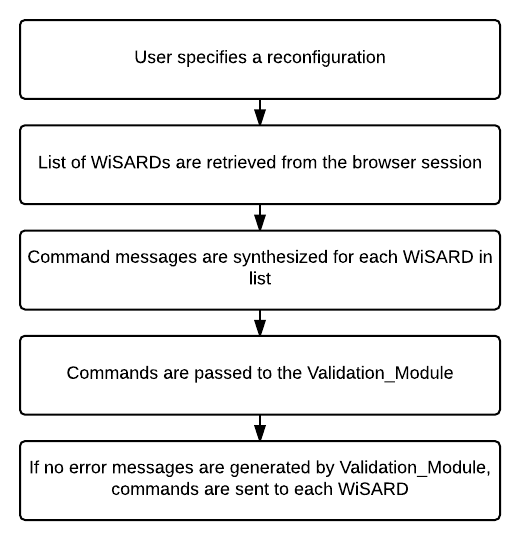
\includegraphics[width=0.6\textwidth]{figures/flow_diagram_cmd_module.png}
	\caption{A flow diagram showing each action the Command Generation Module makes}
	\label{fig:flow_cmd_generator}
\end{figure}

To perform a reconfiguration in WiSARDNet, a specific command is generated and sent to each WiSARD that the change will affect. A command in the WiSARDNet communication protocol consists of multiple components. A hub address and a destination address describe which WSN the command should go to, and which WiSARD in that tree that the command is intended for.\\

These changes include a soft reset on the device, updating a sampling rate, changing a software role or ID, or modifying a task parameter for a transducer. The list of commands that are possible with a WiSARD continues to grow with each new experiment and feature that WiSARDNet supports. It is for this reason that commands need to be implemented in a flexible way such that the current design will not present an obstacle to future developments. In WiSARDNet, a command consists of a payload, an expiration, and a checksum. The payload is the byte stream which contains the command and its parameters the WiSARD will interpret and execute. The expiration is a value which the sender can set to prevent out of date commands from being executed. For example, if a command for some reason takes an hour to traverse the network, it may no longer be relevant and should not be executed. The checksum allows the destination WiSARD to verify that it received the command correctly. A command class encapsulates the elements of a command and provides a foundation to build on for future work.\\

To perform a reconfiguration, a command object is generated for each WiSARD that the change will affect. The change that the user specifies will be enacted for all of the WiSARDs in the list that was added to the session by the servlet. The module loops through each WiSARD and chooses the correct command parameters to include in the payload. Once the command objects have been successfully generated they are sent to the Validation module in a data stucture, similar to the way that the WiSARD browser module provided the WiSARD data structure to the Command module.


% 5.3 Command Validation
% 5.3.1 overview of validation
% - types of validation, UAC and safety
% 5.3.2 Permissions and UAC
% - Describe the design of permissions in the database
% - Remember that this will only be for WiSARDs now but state that the permission resource table could be expanded to anything 
% 5.3.3 Safety Validation
% - Describe use cases and how different commands require different checks
% - Describe design of commands with own validation logic so can be flexible
% - Describe that the validate method is given the database wisard and so all relevant parameters can be obtained through normal database relations?

\section{Validation}
Before commands can be sent out to reconfigure WiSARDs, there are two sets of checks which the commands must pass. First, the Validator module confirms that the user that submitted the commands has appropriate permissions to reconfigure the selected WiSARD nodes. Second, the module assess the commands for their impact on the system, and ensures that none of the changes will cause a WiSARD to misbehave. It is likely that certain WiSARDs will have hardware that is shared between multiple experiments, and a researcher reconfiguring that WiSARD could have adverse on one or more experiments. The procedures that this module performs are shown in Figure \ref{fig:flow_validation_module}. Each of these procedures are described in this section.\\

% flow of execution, validation module
\begin{figure}[H]
	\centering
	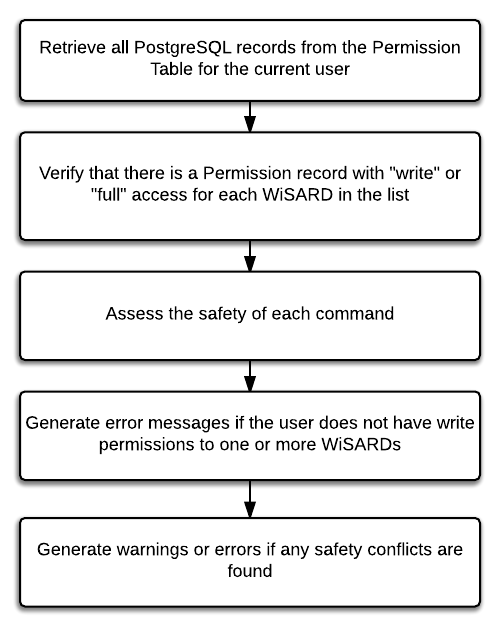
\includegraphics[width=0.6\textwidth]{figures/flow_diagram_validation_module.png}
	\caption{A flow diagram showing each action the Validation Module makes}
	\label{fig:flow_validation_module}
\end{figure}

\subsection{Permissions and User Access Control}
The PostgreSQL database schema prior to this thesis had certain tables which could have been used for user access control, but the schema was not robust. To implement user access control in a flexible way, a better approach was needed. Two core abstractions of the existing database schema are used to design the permissions system for WiSARDNet. The first abstraction is that anyone to whom a permission might be granted is considered a permission entity. The second abstraction is that anything which would need its access restricted is to be considered a permission resource. After applying these two abstractions to the database, the Person and Organization tables are defined as permission entities. Likewise, the Deployment, Site, and Experiment tables are defined as deployment resources. With these two abstractions, granting permission simply becomes a mapping between a permission entity and a permission resource with a value designating the level of access the entity has to the resource.\\ 

Three access levels are used to denote permissions to resources: read, write, and full. Table \ref{tab:permissions} describes what each permission level allows. An important note is that an entity with full access can override changes made by other entities with full access, but a warning message is generated to inform the user of the scenario. In this case, the user should proceed at their own discretion. In the greater context of the user access control paradigm, full permissions also grant a user delete privileges. Even though that use case doesn't directly correlate to the reconfiguration module, the paradigm still supports that feature for other applications. These three permission levels are sufficient to regulate how users  interact with the WiSARDs. This approach to user access control also provides a flexible way to manage other hardware or software resources which might be incorporated into WiSARDNet in the future.\\

\begin{table}[H]
	\centering
	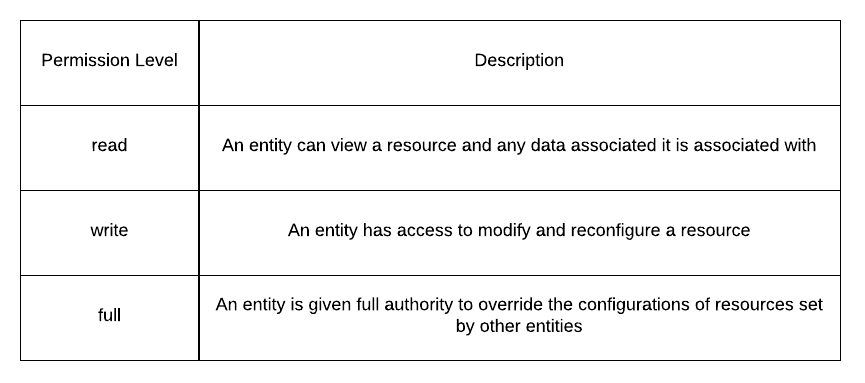
\includegraphics[width=\textwidth]{figures/permission_table.png}
	\caption{A description of each access level an entity can be granted to a resource}
	\label{tab:permissions}
\end{table}

To implement user access control with this approach, three tables were added to the database. First, a Permission Entity table was created to reference the Person and Organization tables. Next, a Permission Resource table was created to reference the Deployment, Experiment, and Site tables. Lastly, a Permission table was created to map records from the Permission Entity table to the Permission Resource table. The references between these tables are governed by foreign key constraints, or referential integrity constraints as they are sometimes referred. Figure \ref{fig:uac_simplified} shows these tables and their foreign key constraints. Each foreign key constraint references the primary key of the table that the arrow points. The unnamed table on the right shows how the schema can be used to manage new resources in the future.

\begin{figure}[H]
	\centering
	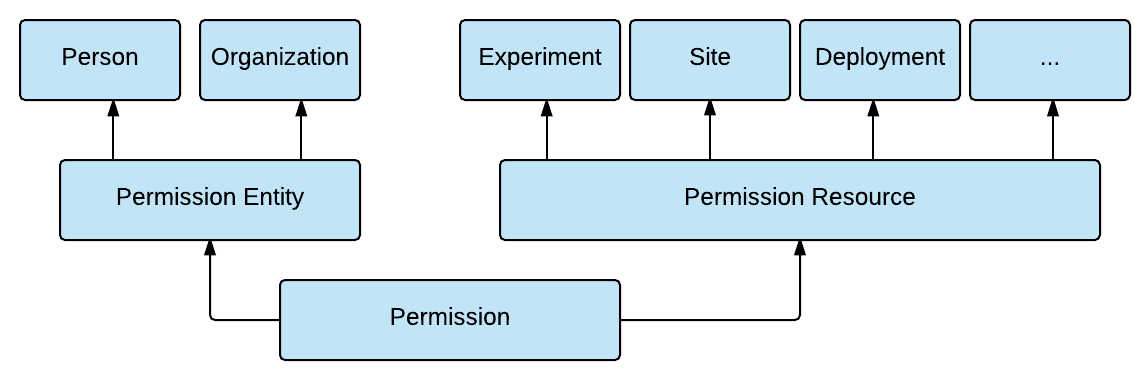
\includegraphics[width=\textwidth]{figures/uac_simplified.png}
	\caption{A diagram that shows how the three new Permission tables are used to create a user access control schema}
	\label{fig:uac_simplified}
\end{figure}

When the validation module receives a data structure of command objects from the command generation module, the software in the validation module first checks that there are no user access violations in any of the commands. This is done by iterating over each command object and performing a lookup to the permission table. The objective is to gather all of the Permission records whose permission entity matches the user that created the commands, and verify that a permission resource with at least write access is present, for the WiSARD in question. If the user is found to have insufficient permissions to execute a command, an error message is generated and added to a queue of messages that is displayed once the validation module has iterated over every command.\\

\subsection{Safety Validation}
 If all of the commands pass the user access permission checks, then the module performs a configuration safety test on each command. The difficulty of the safety check comes from the different types of commands that can be executed, and the diversity of experiments and their needs. It is for this reason that the command class was designed such that each command type will implement its own safety logic. This way, when a new command is developed, the designer can build in a method which will perform a safety check within the context of that method. Figure \ref{fig:cmd_classes} shows the structure of these command classes and how they inherit and override behaviors.\\
 
\begin{figure}[H]
	\centering
	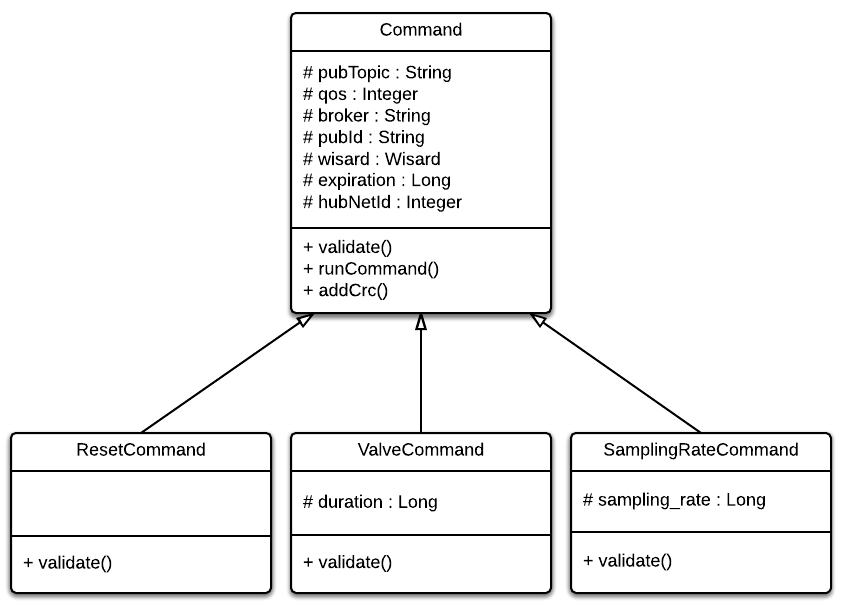
\includegraphics[width=\textwidth]{figures/command_class_diagram.png}
	\caption{A class diagram showing how new commands inherit from their parent class, yet implement their own validate method}
	\label{fig:cmd_classes}
\end{figure}
 
 A practical example of a safety validation method would be a case where a particular command is designed to increase the sampling rate of a particular transducer type on a WiSARD, then an appropriate safety check would be to ensure that the new sampling rate will be a reasonable value. If the user enters a non-numeric value, a negative value, or a value corresponding to a sampling rate which the WiSARDs cannot physically perform, those should result in a failed safety check. Another example is a command to reconfigure a WiSARD that one or more experiments are using. If a configuration change could impact an experiment, a warning message is generated and added to a queue that is shown to the user. In this scenario, the command is not rejected but the user will be warned of the conflict. 

\section{Summary}
Each of the three software modules developed for this thesis serves a distinct role in enabling network reconfiguration. The WiSARD Browser is a flexible module that enables users to search for and select a group of WiSARDs based on a wide range of network state information. The command generator module allows for a user to select a change he/she would like to make to the set of selected WiSARDs, and automatically generate the commands necessary to make them happen. The validation module performs user access control and network safety checks on commands that users create, to ensure that all reconfigurations are made in a way that minimizes the potential for conflicts. The design and implementation of these three modules provides great flexibility to developers who will work on the WiSARDNet platform in the future.
